\section[Supplementary materials: Enhancing sampling]{Supplementary materials for: Enhancing backbone sampling in Monte Carlo simulations using Internal Coordinates Normal Mode Analysis}

\subsection[Are CC and IC modes equivalent?]{Are Cartesian coordinate and internal coordinate normal modes equivalent?}
\label{sec:supp_mat_cc_vs_c}
We have calculated the (Cartesian coordinate) ANM modes and the internal coordinates NMA modes of a set of structures and compared them. Our test set comprises the proteins with PDB ID: 1ubq, 2lzm, 1ex6, 1ddt, 4ake, 1ggg, and the src kinase domain of 1y57. Most of these proteins have been used in NMA benchmarks, as they present wide inter domain movements. We have added two alternative structures for 1ubq and 1y57: 1ubq\_cut, a copy of 1ubq that does not contain the last 3 residues from the C-terminal loop and 1y57\_MD, a randomly picked frame from an MD simulation of 1y57.

The first thing needed in order to compare both sets of modes is to convert the IC modes to CC modes. This can be achieved calculating the Jacobian (J, inverse of Wilson's $B$ matrix) as
\begin{equation}
J_{i,\alpha} = \frac{\partial r_i}{\partial q_\alpha},
\end{equation}
and applying the following equation:
 \begin{equation}
\Delta \vec{r}_{i,\alpha} = \sum_{\alpha}^N \vec{J}_{i,\alpha} v_i^\alpha .
\end{equation}
As all heavy atoms are involved in the calculation of the IC modes and in the conversion, the resulting CC modes will have 3H elements (being H the number of heavy atoms). 

\subsubsection{Collectivity of CC and IC modes}
One of the most compelling features of NMA-based protein simulations is that the modes of lower frequency are able to mobilize big groups of atoms that perform large displacements (i.e. large collective motions). It would be interesting to know if this assumption is true for both models, and if the performance of both is similar. In order to do this we have calculated the first ten ANM and IC NMA modes for and all the structures in our test, modifying the cutoff distance that modulates the density of springs in the elastic network. Then, we have calculated the degree of collectivity of each mode. This gives us information about how the modes change when the elastic network and the shape of the protein change. 

We have also performed a second batch of calculations of IC modes applying the method described by Lu \textit{et al.} \cite{lu_new_2006}. In his work, they add an extra term to the NMA potential, $\nicefrac{\omega}{2} \sum_\alpha (\phi_\alpha - \phi_{\alpha}^0)^2$, where $\omega = 3 min(H_{\alpha\alpha}^0) $. This extra term modifies the Hessian diagonal, presumably lowering the so-called ``tip effect'' problem.

To quantify the differences of collectivity, we will calculate the degree of collectivity. This measure, first proposed by Bruschweiler \cite{bruschweiler_collective_1995}, quantifies the number of atoms that are affected by a mode and the relative magnitude of the induced displacement. Its value can be calculated as

\begin{equation}
\kappa_i = \frac{1}{N} exp \left( -\sum^N_j \alpha \Delta R_j^2 log \left( \alpha \Delta R_j^2 \right) \right),
\end{equation}

where $N$ is the number of atoms and $\Delta R_j$ is the atomic displacement described by mode $i$ on atom $j$. 
The degree of collectivity is proportional to the exponential of the ``information entropy'' embedded in vector $\Delta R$ \cite{tama_conformational_2001}. Its lower and upper bound is known ($N^{-1}$ and 1 respectively). This allows us to normalize its value in the range $[0,1]$, meaning 1 that the conformational change the mode produces is maximally collective.

As we can see in Fig. \ref{fig:collectivities_per_cutoff}, the average collectivities of the CC modes are always lower than their IC counterparts. Furthermore, the degree of collectivity seems to decline as the cutoff varies and the elastic network becomes more dense. Conversely, the IC modes remain almost unaffected by the changes of the elastic network. It is worth noting that the ones calculated using the Hessian modification method have slightly higher values of collectivity and are, again, almost immune to the EN changes. 

\begin{figure}
\includegraphics[width=\linewidth, height=\textheight, keepaspectratio]{avg_collectivities_per_cutoff}
\caption{Degree of collectivity for each structure and calculation method. .}
\label{fig:collectivities_per_cutoff}
\end{figure}

From the plot we can see that 9 $\AA$ is a good choice for the cutoff: it yields good collectivity values and it is in agreement with the conclusions of other studies \cite{zheng_anharmonic_2010}.

\begin{figure}
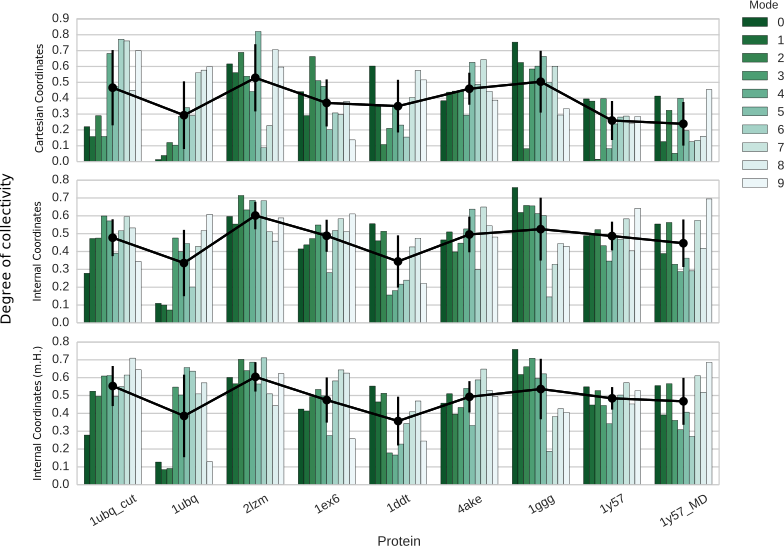
\includegraphics[width=\linewidth, height=\textheight, keepaspectratio]{cut_9_avg_coll}
\caption{Detailed study of the degree of collectivity per mode, structure and method. Cutoff has been set to 9 \angstrom. The Hessian modification method (m.H.) produces only slight improvements, generally concentrated in higher frequency modes.}
\label{fig:cut_9_avg_coll}
\end{figure}

The detailed view of mode collectivities for a cutoff of 9 \angstrom  is shown in Fig. \ref{fig:cut_9_avg_coll}. We can see how the collectivity of IC modes is higher, especially that of the lower frequency modes. The differences between 1ubq\_cut and 1ubq are of particular interest. In these two cases, the collectivity values of the lower frequency modes of 1ubq are pretty small for all three methods, and they increase perceptibly in 1ubq\_cut. This must be caused by the only difference between these two structures: the appearance of the C-terminal loop. The structure with the loop (1ubq) is severely suffering from the ``tip effect'' due to the flexibility of the final loop, perfectly illustrating how this effect can worsen the collectivity of the modes.  

From the analyses performed on this data set, we can conclude that IC modes have higher collectivity, and  that this collectivity is more robust to changes in the elastic network.  

\subsubsection{Comparison between the CC and IC mode spaces}

We also wonder to which extent the mode space spanned by the CC and IC modes is similar. To this end we will use two measures: the cumulative overlap and the root mean square inner product (RMSIP). Both of them are based on the mode overlap operation, which measures the projection of one mode over the other. It can be calculated as:
\begin{equation}
O_{ij} = \frac{\left | P_i . M_j \right |}{{\Arrowvert P_i\Arrowvert}{\Arrowvert M_j\Arrowvert}} .
\end{equation}
Its value ranges from 0 to 1, meaning 1 a perfect overlap.  

The Cumulative overlap \cite{yang_close_2008} measures to which extent a range of modes can capture the motion of a single mode. It is calculated as
\begin{equation}
CO_i(k)= (\sum_{j}^{k} O_{ij}^2)^\frac{1}{2},
\end{equation}
where $i$ is the mode we are checking and $[j,k]$ is the range of modes we will use to explain the first. Its value is, again, in the range from 0 to 1, meaning 1 a perfect match (assuming perfect orthogonality of the modes).   

Finally, the RMSIP \cite{amadei_convergence_1999,leo-macias_analysis_2005} measures how the normal mode space spanned by a range of modes overlaps with another range of modes. It is calculated as  
\begin{equation}
RMSIP(l,m) = \left( \frac{1}{l} \sum_{i=1}^l \sum_{j=1}^m {(P_i.M_j)}^2 \right )^\frac{1}{2} .
\end{equation}
Its value is independent of the mode order and ranges from 0 to 1, meaning 1 that both normal mode spaces are identical.

It is important to note that the modes coming from the IC conversion and PELE ANM model are defined for a different number of atoms (all heavy atoms in the first case, $C_\alpha$s in the second) and, therefore, they represent very different mode spaces. In order to make the comparisons possible, we need to calculate the ANM modes for all heavy atoms.

The cumulative overlaps shown in Figs. \ref{fig:avg_cum_overlap_per_cutoff} and \ref{fig:cut_9_cumulative_overlap} indicate that both mode spaces can explain each other successfully, being 1ubq, 1ubq\_cut and 1y57\_MD the only exceptions. In general, increasing the cutoff makes the differences between mode spaces more noticeable. The calculations performed with cutoff distance equal to 9 \angstrom (Fig. \ref{fig:cut_9_cumulative_overlap}), show that lower frequency modes are generally the ones that find a best correspondence with the modes of the other space.

\begin{figure}
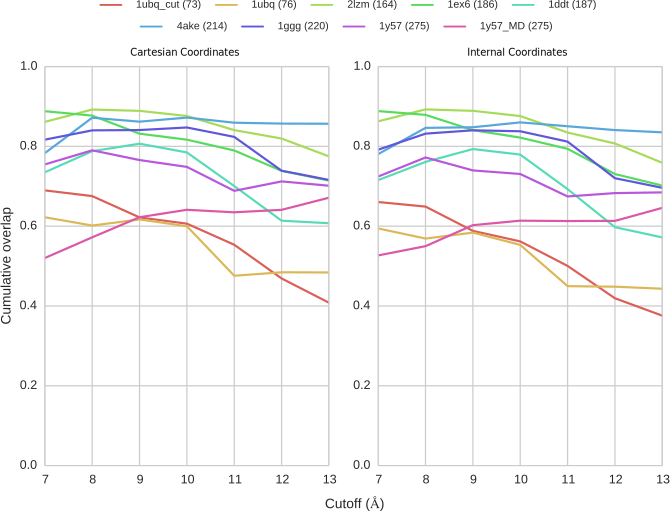
\includegraphics[width=\linewidth, height=\textheight, keepaspectratio]{avg_cum_overlap_per_cutoff}
\caption{ Average cumulative overlap for different cutoff distances, methods, and structures in our test set. Standard deviations are not shown for the sake of clarity.}
\label{fig:avg_cum_overlap_per_cutoff}
\end{figure}
 
\begin{figure}
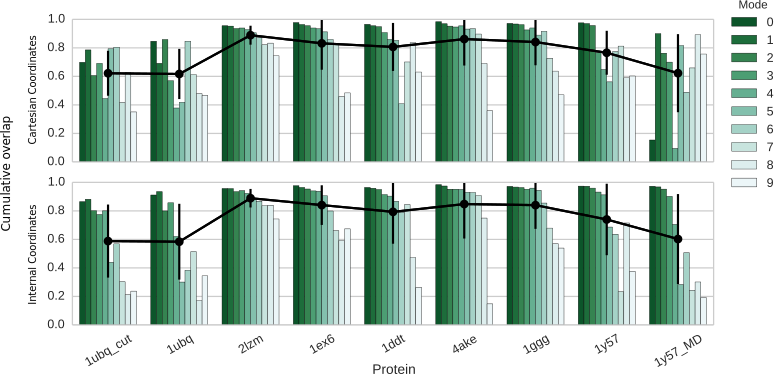
\includegraphics[width=\linewidth, height=\textheight, keepaspectratio]{cut_9_cumulative_overlap}
\caption{Detailed study of the cumulative overlap per mode, structure and method. Cutoff has been set to 9 \angstrom. In general, the rightmost modes (higher frequencies) are the ones with worst overlap.} 
\label{fig:cut_9_cumulative_overlap}
\end{figure}

Regarding the RMSIP for the modes calculated using a cutoff distance of 9 \angstrom, the mode space overlap is higher for the subspace of the low frequency modes, and decreases when more high frequency modes are added to the calculation (see Fig. \ref{fig:cut_9_rmsip_per_mode_range}), which correlates well with the observations made for Fig. \ref{fig:cut_9_cumulative_overlap}.

\begin{figure}
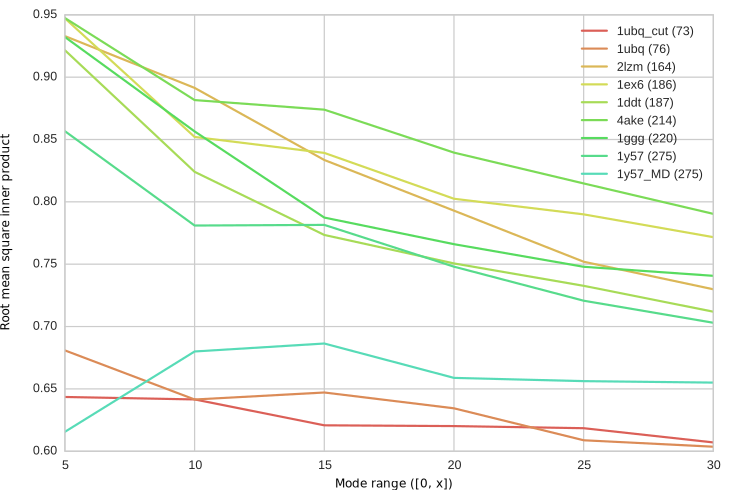
\includegraphics[width=\linewidth, height=\textheight, keepaspectratio]{cut_9_rmsip_per_mode_range}
\caption{RMSIP of CC and IC mode spaces. The x-axis shows the upper limit of the mode space tested (e.g, 10 means that the first ten modes are to be used to obtain the RMSIP). Both spaces look to be very similar, at least for the 5 lowest frequency modes. The similarities decrease as we move to modes of higher frequencies, with the only exceptions already commented in the cumulative overlap study.}
\label{fig:cut_9_rmsip_per_mode_range}
\end{figure}
